%http://www.prisma-statement.org/PRISMAStatement/

% 1 •
% •
% TITLE
% TITLE
% •
% Identify the report as a systematic review in the title.
% Report an informative title that provides key information about the main objective or question the review addresses (e.g. the population(s) and
% intervention(s) the review addresses).
% Consider providing additional information in the title, such as the method of analysis used, the designs of included studies, or an indication that the review
% is an update of an existing review, or a continually updated (“living”) systematic review.

% \section{\MakeUppercase{Систематичний огляд застосування штучних нейронних мереж для генерацiї текстового контенту (2022-2024)}}

\clearpage

\section{\MakeUppercase{ТЕОРІЯ Й ПРАКТИКА ДИФЕРЕНЦІЙОВАНОГО НАВЧАННЯ УЧНІВ ЛІЦЕЇВ}}
\subsection{Навчання учнів інформаційної безпеки як педагогічна проблема\label{sec1.1}}

%з метою визначення сучасного стану досліджень у галузі навчання інформаційній безпеці учнів шкіл було проведено бібліографічний пошук за матеріалами, які представлені в науково-метричній базі Scopus. 



Стрімкий розвиток інформаційних технологій та їх глибока інтеграція в усі сфери життя сучасного суспільства актуалізує проблему навчання учнів закладів загальної середньої освіти основам інформаційної безпеки. Цифрова трансформація освітнього процесу, масовий перехід на дистанційне навчання під час пандемії COVID-19, а також зростання кіберзагроз створюють нові виклики для педагогічної спільноти.

З метою визначення сучасного стану досліджень у галузі навчання інформаційній безпеці учнів було проведено комплексний бібліографічний аналіз наукових публікацій, представлених у науково-метричній базі Scopus. Пошук здійснювався за запитом: \textit{(``learning'' OR ``education'') AND (``information security'' OR ``Cybersecurity'') AND ``school''}, що дав змогу ідентифікувати 585 релевантних публікацій.

Для аналізу та візуалізації бібліографічних даних було використано програмне забезпечення VOSviewer /cite{VOSviewer}, яке надає інструменти для створення карт відповідності ключових слів та виявляти тематичні кластери в масиві наукових публікацій. Аналіз проводився за такими параметрами:
\begin{itemize}
    \item тип аналізу: відповідність ключових слів (co-occurrence);
    \item одиниця аналізу: усі ключові слова (all keywords);
    \item метод підрахунку: повний підрахунок (full counting);
    \item мінімальна кількість зустрічей ключового слова: 10.
\end{itemize}

З початкових 3407 ключових слів після застосування порогового значення було відібрано 71 термін, які сформували основу для кластерного аналізу.


Аналіз географічного розподілу публікацій виявив домінування англомовних країн у дослідженнях з навчання інформаційній безпеці в школах. Країни, які є лідерами за кількістю публікацій, зазначені в таблиці~\ref{leaders}

\begin{table}[h] 
\centering
\caption{Географічний розподіл публікацій з навчання інформаційній безпеці.}
\label{leaders}
\begin{tabular}{|l|c|c|c|}
\hline
\textbf{Країна} & \textbf{Документи} & \textbf{Цитування} & \textbf{Сила зв'язків} \\
\hline
США & 215 & 1285 & 17 \\
Австралія & 10 & 102 & 11 \\
Велика Британія & 24 & 238 & 9 \\
Канада & 7 & 54 & 7 \\
Південна Африка & 14 & 80 & 7 \\
Німеччина & 8 & 23 & 6 \\
Індія & 9 & 71 & 6 \\
\hline
\end{tabular}
\end{table}


Кластерний аналіз дав змогу виділити п'ять основних тематичних напрямів досліджень у галузі навчання інформаційній безпеці учнів (рис.~\ref{VOSmap}):

\begin{figure}[h]
    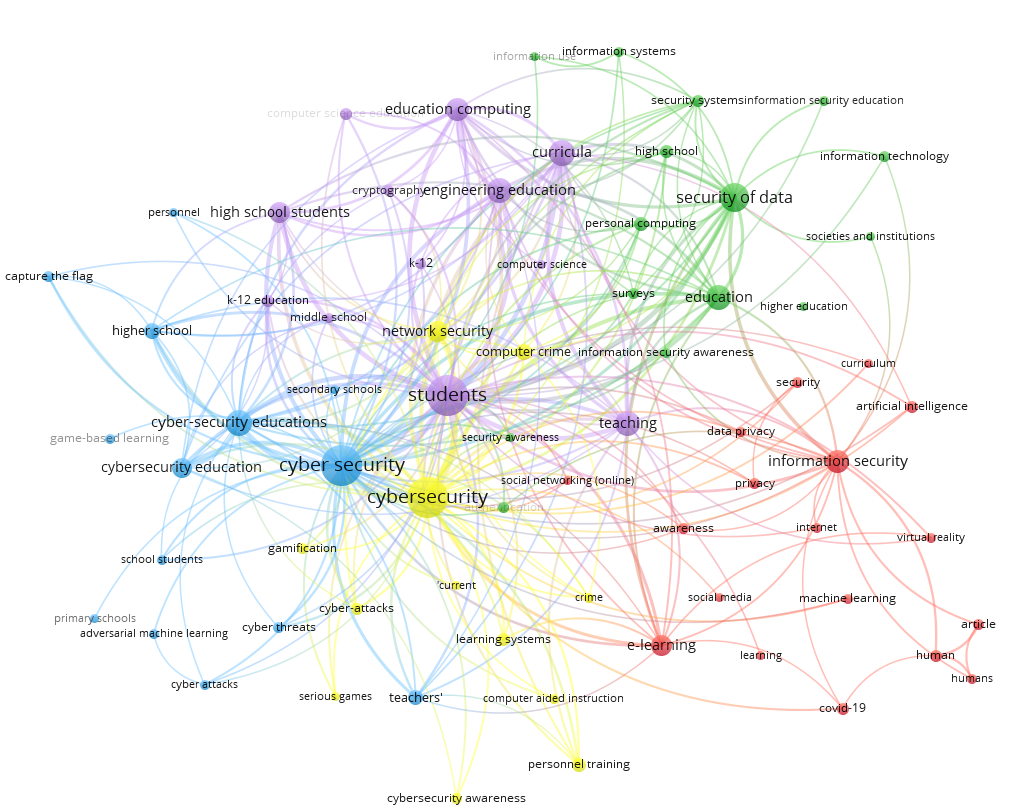
\includegraphics[width=\linewidth]{imgchap1/VOSmap.png}
    \caption{Кластерний аналіз за тематичними напрямами досліджень}
    \label{VOSmap}
\end{figure}

\begin{enumerate}[label=--] % дописать
\item 
\textbf{кластер 1: ``Інформаційні технології та їхній вплив на суспільство''} (червоний) -- об'єднує дослідження, присвячені впливу сучасних технологій на освітній процес та суспільство в цілому. Ключовими термінами є: \textit{artificial intelligence} (середній рік публікації -- 2021.4), \textit{machine learning} (2022.1), \textit{e-learning} (52 появи), \textit{data privacy}, \textit{virtual reality}, \textit{social media}. Високий середній рік публікацій свідчить про актуальність та новизну досліджень у цій сфері;


\item 
\textbf{кластер 2: ``Освіта та обізнаність у сфері інформаційної безпеки''} (зелений) -- наукові праці, що зосереджені на формальній освіті та підвищенні обізнаності в питаннях інформаційної безпеки. Основні терміни: \textit{information security awareness} (45 зв'язків), \textit{information security education} (12 появ), \textit{security of data} (99 появ, 425 зв'язків), \textit{authentication}, \textit{higher education}. Значна кількість зв'язків підкреслює центральну роль цієї тематики в загальному масиві досліджень;

\item 
\textbf{кластер 3: ``Навчання кібербезпеці в освітніх закладах''} (синій) --
найпотужніший кластер за кількістю зв'язків, присвячений практичним аспектам навчання кібербезпеці. Провідні терміни: \textit{cyber security} (195 появ, 1008 зв'язків), \textit{cybersecurity education} (49 появ), \textit{capture the flag}, \textit{game-based learning}. Присутність ігрових методів навчання вказує на інноваційні підходи до викладання кібербезпеки;

\item 
\textbf{кластер 4: ``Тренування та освіта персоналу в галузі кібербезпеки''} (жовтий) --
 охоплює питання професійної підготовки та підвищення кваліфікації. Ключові терміни: \textit{cybersecurity} (195 появ, 862 зв'язки), \textit{computer crime} (середнє цитування -- 14.3), \textit{personnel training}, \textit{serious games}, \textit{gamification}. Високі показники цитування свідчать про значущість тематики в науковій спільноті;

\item 
\textbf{кластер 5: ``Освіта в комп'ютерних науках та інженерії''} (фіолетовий) -- представляє академічні аспекти комп'ютерної освіти. Основні терміни: \textit{curricula} (76 появ), \textit{students} (190 появ, 1008 зв'язків), \textit{computer science education}, \textit{engineering education}, \textit{k-12 education}. Високі показники для терміну ``students'' підкреслюють студентоцентрований підхід у дослідженнях.
\end{enumerate}

Аналіз хронологічного розподілу публікацій виявив, що активне дослідження проблем навчання інформаційній безпеці в закладах загальної середньої освіти розпочалося у 2021--2022 роках. Це пов'язано з масовим переходом на дистанційне навчання під час пандемії COVID-19 та зростанням кіберзагроз в освітньому середовищі.


Сучасні дослідження демонструють зміщення акценту від традиційних методів навчання до інноваційних підходів:

\begin{enumerate}[label=--] % дописать
    \item \textit{гейміфікація освітнього процесу} -- використання ігрових механік для підвищення мотивації та залученості учнів. Терміни ``gamification'', ``serious games'', ``game-based learning'' мають високі показники цитування та актуальності;
    
    \item \textit{змагання CTF (Capture The Flag)} -- практично-орієнтований метод навчання через вирішення реальних задач з кібербезпеки в змагальному форматі. Середній рік публікацій -- 2022.8, що свідчить про новизну підходу;
    
    \item \textit{персоналізоване навчання} -- адаптація освітнього контенту до індивідуальних потреб та рівня підготовки учнів з використанням технологій штучного інтелекту та машинного навчання;
    
    \item \textbf{симуляційне навчання} -- створення безпечного віртуального середовища для відпрацювання навичок протидії кіберзагрозам.
\end{enumerate}


Аналіз зв'язків між кластерами виявив високий рівень міждисциплінарності досліджень. Терміни ``cyber-security educations'' та ``cybersecurity education'' з'являються одночасно в кількох кластерах, що свідчить про інтеграцію технічних, педагогічних та соціальних аспектів проблеми.
На основі проведеного аналізу можна виділити особливості навчання інформаційній безпеці:

\begin{enumerate}[label=--] % дописать
    \item \textit{динамічність предметної області} -- швидка зміна технологій та загроз вимагає постійного оновлення навчальних програм та методичних матеріалів;
    
    \item \textit{обмежена кількість кваліфікованих педагогічних кадрів} -- необхідність підготовки вчителів, які володіють як технічними знаннями, так і педагогічними методиками викладання кібербезпеки;
    
    \item \textit{вікова диференціація} -- необхідність розробки навчальних програм для різних вікових груп;% (primary schools, middle school, high school, k-12);
    
    \item \textbf{практична спрямованість} -- забезпечення балансу між теоретичними знаннями та практичними навичками безпечної поведінки в цифровому середовищі.
\end{enumerate}


Проведений бібліографічний аналіз свідчить про зростання наукового інтересу до проблем навчання учнів інформаційній безпеці. Виявлені тематичні кластери демонструють комплексний характер проблеми, що охоплює технологічні, педагогічні, психологічні та соціальні аспекти.

Домінування термінів ``cyber security'' (195 появ) та ``students'' (190 появ) з найвищими показниками зв'язків підкреслює центральну роль учнівської аудиторії в дослідженнях кібербезпеки. Поява інноваційних методів навчання, таких як гейміфікація, CTF-змагання та симуляційне навчання, свідчить про пошук ефективних педагогічних рішень для формування культури кібербезпеки в молодого покоління.

Перспективними напрямами подальших досліджень є розробка диференційованих методик навчання інформаційній безпеці з урахуванням вікових особливостей учнів, створення інтегрованих навчальних програм, що поєднують технічні та гуманітарні аспекти кібербезпеки, а також підготовка педагогічних кадрів для ефективного викладання цієї дисципліни в закладах загальної середньої освіти.


\subsection{Диференційоване навчання в середній освіті}

Поняття диференційованого навчання розвивалося від простого групування учнів до гнучкого пристосування педагогічних елементів до їхніх потреб. Класичною науковою працею в галузі диференційованого навчання, яка зазначає сучасний погляд міжнародної освітянської спільноти на проблему, є монографія Керол Енн Томлінсон ``Як диференціювати навчання в класах зі змішаними здібностями''  \cite{Tomlinson2001}. Автор розуміє диференційоване навчання як ``упорядкування викладання для задоволення індивідуальних потреб'' учнів \cite{Tomlinson2001}. Це означає, що диференціація~-- це проактивна, якісна та орієнтована на учня філософія, а не просто набір хаотичних дій. Виділяють чотири основні елементи навчального процесу, які вчитель може адаптувати для задоволення індивідуальних потреб учнів \cite{Tomlinson2001}: 
\begin{enumerate} [label=\arabic*)]% дописать
\item зміст (content)~-- різні шляхи, якими учні отримують доступ до ключових концепцій та інформації~-- використання різних матеріалів (різного рівня складності), варіативність джерел (відео, аудіо, текст);
\item процес (process)~-- різні види діяльності, якими учні опрацьовують і осмислюють ідеї~-- робота в різних групах (за рівнем готовності, інтересами), надання вибору завдань, різні стилі навчання (візуальний, аудіальний, кінестетичний);
\item продукт (product)~-- різні шляхи, якими учні демонструють своє розуміння та знання~-- можливість створити есе, презентацію, постер, макет або усний звіт для підсумкової оцінки;
\item середовище (environment)~-- створення сприятливої та гнучкої атмосфери в класі, яка підтримує індивідуальні потреби~-- гнучке розташування меблів, встановлення правил роботи в групах, створення теплого клімату співпраці.
\end{enumerate}

Згідно \cite{Tomlinson2001} адаптація (диференціація) повинна базуватися на трьох основних характеристиках кожного учня:
\begin{enumerate} [label=\arabic*)]% дописать
\item
рівень готовності (readiness) -- рівень знань, навичок та розуміння, які учень має на даний момент для роботи з конкретним навчальним матеріалом: диференціація за готовністю регулює складність та темп;
\item
інтереси (interests) -- теми, об'єкти або сфери, які викликають у дитини природну цікавість та бажання навчатися: диференціація за інтересами підвищує мотивацію та залученість;
\item
профіль навчання (learning profile) -- переваги учня щодо стилю навчання (наприклад, візуальний, кінестетичний), групової роботи, та впливу середовища: диференціація за профілем навчання регулює спосіб викладання.
\end{enumerate}

Слід наголосити, що у центрі моделі К. Томлінсон знаходиться учень і його успіх, що досягається завдяки гнучкості навчального процесу.

Термінологічний апарат стосовно диференційованого навчання детально пропрацьований у вітчизняних науково-педагогічних дослідженнях \cite{Білик2017, ШАРОВ2021, Шевчук_2020, Пісоцька2022}. 

Для визначення сучасних вітчизняних тенденцій у галузі диференційованого навчання в закладах загальної середньої освіти було побудовано запит на сайті  проєкту ``Ініціатива з відкритого доступу до українського наукового контенту (OUCI)'', що забезпечує доступ до бібліографічних даних наукових публікацій, які використовують сервіс Cited-by від Crossref та підтримують Initiative for Open Citations: 

\begin{verbatim}
https://ouci.dntb.gov.ua/?q=диференційоване+навчання
&f_pub_type=journal-article
&f_pub_year=2025%7C2023%7C2024%7C2021%7C2022
&f_specialty=014
\end{verbatim}

Згідно цього запиту розглядаємо статті в наукових журналах, які стосуються диференційованого навчання, відповідають спеціальності 014 (Середня освіта) та опубліковані в період із 2021 по 2025 рік. Особливістю побудови запитів на сайті є автоматичне варіювання словоформ, що значно полегшує пошук українською мовою. Відповідно до дослідницького завдання, а саме визначення актуальних підходів до організації диференційованого навчання в закладах середньої освіти, було сформульовано умови включення публікацій до розгляду:
\begin{enumerate}[label=\arabic*)]
    \item наявність інформації про способи організації диференційованого навчання;
    \item наявність прикладів методики диференційованого навчання;
    \item наявність інформації про психолого-педагогічні умови диференціації навчання.
\end{enumerate}


Умовами виключення є:
\begin{enumerate} [label=\arabic*)]% дописать
\item невідповідність матеріалу середній освіті;
\item відсутність інформації про диференційоване навчання щодо формування знань і розумових умінь;
\item повторення даних попередніх публікацій;
\item відсутність повного тексту статті у відкритому доступі.
\end{enumerate}

За запитом до бази даних на 31 жовтня 2025 року було отримано 22 джерела. 
Результати попереднього аналізу зазначених публікацій щодо умов включення до огляду та умов виключення з огляду подано в таблиці~\ref{conditions}. 

% \begin{table}[h]
%\centering
{\footnotesize
\setlength \tabcolsep {0.4\tabcolsep}
\begin{longtable}{|p{0.35\textwidth}|p{0.24\textwidth}|p{0.24\textwidth}|p{0.12\textwidth}|}
\caption{\normalsize Умови включення знайдених публікацій до розгляду.}
\label{conditions}
\\
\hline
\hfil \textbf{Назва, doi} & \textbf{Умови включення до огляду} & \textbf{Умови виключення з огляду} & \textbf{Висновок щодо включення до огляду} \\
\hline
\multicolumn{1}{|c|}1 &  
\multicolumn{1}{c|}2  & 
\multicolumn{1}{c|} 3  & 
\multicolumn{1}{c|} 4  \\
\hline
\endfirsthead % Заголовок для першої сторінки

\multicolumn{4}{r}{{Продовження табл. \thetable}} \\
\hline
\multicolumn{1}{|c|}1 &  
\multicolumn{1}{c|}2  & 
\multicolumn{1}{c|} 3  & 
\multicolumn{1}{c|} 4  \\
\hline
\endhead % Заголовок для наступних сторінок

%\multicolumn{4}{r}{\textbf{Закінчення табл. \thetable}} \\
%\hline
\endlastfoot % Вміст для ОСТАННЬОЇ СТОРІНКИ

Theoretical principles of differentiated work of primary school students: main aspects, 10.32626/2309-9763.2020-29-157-167 & 
1~-- розглядається диференціація навчальної діяльності & 
1~-- спрямовано на початкову школу & 
Ні \\
\hline
{Диференціація та індивідуалізація освіти в сучасному ЗВО: можливості інформаційного середовища}, 10.32689/ maup.ped.2024.3.2 & 
1~-- розглядається диференціація навчальної діяльності & 
1~-- спрямовано на вищу освіту & 
Ні \\
\hline
{Current state of training of future teachers professional training for innovative pedagogical activities in educational theory}, 10.31376/2410-0897-2024-2-55-10-19 & 
- & 
1~-- спрямовано на вищу освіту  & 
Ні \\
\hline
{Особливості підготовки майбутніх учителів природничих спеціальностей на засадах диференціації та індивідуалізації навчання}, 10.24919/2308-4634.2024.301830 & 
1~-- розглядається диференціація навчальної діяльності & 
1~-- спрямовано на вищу освіту  & 
Ні \\
\hline
{До проблеми оцінювання навчальних досягнень учнів гімназій у компетентнісному вимірі},
10.32405/2411-1309-2024-32-66-82
& 
-
& 
2~-- не містить інформації про диференційоване навчання. Містить вимоги вимоги до оцінювання, які диференційовано
 & 
Ні
\\
\hline
 Методичні підходи, реалізовані у підручнику з математики для учнів 6 класів (за підручником «Математика. 6 клас» Світлани Скворцової та Катерини Нєдялкової),
10.32405/2411-1317-2023-3-217-226
 & 
1 + 2~-- Тренувальні завдання диференційовано за трьома рівнями складності. Проєктне навчання втілюється через виконання школярами проєктів різної тематики: «Поглиначи часу», «Волонтерська діяльність», «Подорож річками України», «Український борщ», «Золотий перетин», «Подорож повітряним океаном», «Зелений одяг планети», «Світ професій і математика».
 & 
-
 & 
Так~\cite{Скворцова_Нєдялкова_2023}
\\
\hline
{Значення штучного інтелекту у вивченні іноземних мов},
10.26661/2786-5622-2024-1-03
 & 
1~-- цифровизація (ШІ) робіть процес здобуття знань персоналізованим і диференційованим

 & 
1~-- орієнтовано на вищу школу
 & 
Ні
\\
\hline
{Шкільний підручник з української літератури як інструмент формування медіаграмотності сучасних учнів},
10.15330/obrii.59.2.49-54
 & 
-
 & 
2~-- у статті тільки згадується, що підручник має рубрику ``диференційовані завдання'' проте суть цих завдань і принципи диференціації не повідомлюються 
 & 
Ні
\\
\hline
 Потенціал підручника «досліджуємо історію і суспільство» у формуванні екологічної компетентності учнів 6 класу,
10.32405/2411-1309-2023-31-211-222
& 
-
& 
2~-- автори зазначають, що ``Зміст завдань дає змогу використовувати їх диференційовано, організувати самостійну
/ парну / групову роботу учнів, досягати очікуваних результатів навчання'', проте принципи диференціації  не наводяться, приклади завдань не супроводжуються коментарями, в чому може полягати диференціація
& 
Ні
\\
\hline
{Проблеми та перспективи розвитку інклюзивної освіти в умовах реформування освітньої галузі України},
10.33216/2220-6310-2021-102-3-85-94
& 
1~-- впровадження диференційованих методів та технологій навчання особистісно-орієнтованого спрямування із урахуванням індивідуальних особливостей дитини — інклюзивна освіта
 & 
-
 & 
Так~\cite{Гайдаєнко_Рашидов_2021}
\\
\hline
{Роль електронного портфоліо вчителя як освітнього ресурсу в навчально-методичному забезпеченні процесу подолання освітніх втрат учнів},
10.32405/2411-1309-2024-32-299-305
& 
1~--  учитель розробляє диференційовані завдання, які допоможуть учням поступово нарощувати рівень своєї освітньої самостійності 
 & 
-
& 
Так~\cite{Трубачева_Мішеніна_Коник_2024}
\\
\hline
Formation of an integrated course for the 5–6th grades as a component of integral natural science education,
10.32626/2309-9763.2020-29-171-186
& 
1~-- диференційоване вивчення окремих предметів
 & 
-
& 
Так~\cite{Засекіна_2020}
\\
\hline
{Formation of an integrated course for the 5–6th grades as a component of integral natural science education},
10.32405/2411-1317-2021-4-65-76
& 
-
& 
2~-- стаття присвячена цифрової трансформації, диференціація тільки згадується
 & 
Ні
\\
\hline
{Directions for optimization of the corrective-developmental process in speech therapy groups},
10.31494/2412-9208-2023-1-3-183-193
& 
1~-- диференційована роботи під час фронтального корекційно-розвиткового навчання в логопедії
 & 
1~-- діти дошкольного віку
 & 
Ні 
\\
\hline
{Content, forms and methods of work on the of physical education of primary school students in the socio-cultural environment},
10.31376/2410-0897-2023-2-52-248-254
& 
-
& 
1~-- початкова школа
 & 
 Ні
\\
\hline
{Інформаційно-комунікаційні технології як засіб формування лінгводидактичної компетентності майбутніх учителів початкових класів},
10.33407/itlt.v82i2.3288
& 
-
& 
1~-- вища школа
 & 
Ні
\\
\hline
{Strategie of social adaptation of preschool students with speech disorders in the conditions of inclusive education},
10.31494/2412-9208-2023-1-3-194-202
& 
-
& 
1~-- дошкільна освіта
& 
Ні
\\
\hline
{\small Морфофункціональні показники учнів як чинник диференціації корекційно-педагогічного підходу в ортопедагогіці},
10.31865/2077-1827.2(108) 2025.340168
& 
- 
& 
 2~-- розглядаються показники учнів середнього шкільного віку з незначними порушеннями опорно-рухового апарату як ключовий чинник диференціації корекційно-педагогічного підходу в ортопедагогіці. Мова йде про формування опорно-рухового апарату, а не про формування системи знань та розумових умінь

 & 
Ні
\\
\hline
{Теоретичні аспекти використання педагогічних інновацій у післядипломній педагогічній освіті},
10.26661/2786-5622-2023-1-19
& 
-
& 
2~-- диференціоване навчання тільки згадується
 & 
Ні 
\\
\hline
{Перспективи комплексного використання засобів спортивних ігор у фізичному вихованні учнів початкових класів закладів загальної середньої освіти},
10.32782/olimpspu/2024.1.9
& 
-
& 
1~-- початкова школа 
& 
Ні
\\
\hline
{Міждисциплі-нарний контент понять «інтенція», «мовленнєва інтенція» у логокорекційних системах сучасної логопедії},
10.31392/npu-nc.series 19.2023.44.09
& 
-
& 
1~-- діти із тяжкими порушеннями мовлення
 & 
 Ні
\\
\hline
{Особливості організації інклюзивного фізичного виховання в умовах нової української школи},
10.24195/ olympicus/2025-2.19
& 

 & 
2~-- автори зазначають, що інклюзивне фізичне виховання вимагає застосування диференційованих вправ та адаптованого обладнання. Отже мова не йде про формування знань та розумових умінь 
 &
 Ні
\\
\hline
%\normalsize
\end{longtable}
}

За результатами проведеного аналізу можна зробити висновок, що попри значного інтересу до диференційованого навчання акцент останніх наукових праць із цього напряму більше спрямований на фізичне виховання, початкову та вищу школу. Щодо середньої освіти, то маємо зазначити інтерес до інклюзивного навчання та диференційованого підходу. Так у праці~\cite{Гайдаєнко_Рашидов_2021} зазначається важливість «... впровадження  диференційованих  методів  та  технологій  навчання особистісно-орієнтованого    спрямування    із    урахуванням індивідуальних особливостей дитини». Проте конкретних рекомендацій про особливості диференціації відповідного навчального матеріалу або процесу та підходи до діагностики з метою рекомендування того чи іншого матеріалу не наводяться~-- автори закликають до активізації досліджень у цьому напрямі. 

Як напрям диференціації навчання C. Трубачева, Т. Мішеніна, О.~Коник розглядають наповнення портфоліо вчителя: «Важливою складовою портфоліо може бути постійно оновлюваний розділ для учнів, з диференційованими завданнями для вивчення найбільш актуального предметного матеріалу, який допоможе учням у подоланні освітніх втрат~...»~\cite{Трубачева_Мішеніна_Коник_2024}. На думку авторів, диференційовані завдання мають сприяти підвищенню самостійності учнів. Отже напрямом диференціації є характер та детальність інструкцій, які отримує учень~\cite{Трубачева_Мішеніна_Коник_2024}. Автори, також, пов'язують рівень самостійності із рівнем розумової діяльності, яку мають здійснити учні під час виконання завдань. Низькому рівню самостійності відповідають завдання переважно репродуктивного характеру, «завдання для учнів із середнім рівнем самостійності повинні мати продуктивний характер з додаванням опорних схем до їх виконання»~\cite{Трубачева_Мішеніна_Коник_2024}. Для визначення рівня самостійності учнів автори пропонує такі показники: планування навчальної діяльності, виконавча робота, уміння логічно аналізувати та систематизувати навчальний матеріал, уміння піддавати рефлексії шлях виконання завдання та отримані результати, уміння працювати з електронними освітніми платформами та додатками~\cite{Трубачева_Мішеніна_Коник_2024}. Маємо зазначити, що проблему управління самостійною роботою було розглянуто детальніше у працях Л.~Білоусової і Л.~Колгатіної~\cite{Білоусова_2019}. А саме, окрім диференціації інструкцій щодо постановки завдань було підкреслено важливість диференціації допомоги в процесі виконання завдань учнями на всіх етапах від постановки завдання до аналізу результатів і підготовки звіту, а також, диференціації середовища, в якому виконується завдання (наявність та ступінь структурованості ресурсів, потрібних для виконання завдання)~\cite{Білоусова_2019}. Такий підхід дає змогу навчати учнів із низькім рівнем самостійності виконувати завдання дослідницького характеру через поступовий перехід від прямого управління їх самостійною роботою до співуправління, побічного управління, самоуправління~\cite{Bilousova_Kolgatina_Kolgatin_2023}.  

Т.~Засєкіна зазначає необхідність диференціації під час побудови системи природничої освіти для учнів 5-6 класів~\cite{Засекіна_2020}. Авторка пропонує розроблення пропедевтичного природознавчого курсу, який має бути опорою для подальшого диференційованого вивчення деяких природничих предметів, що відтворює класичну логіку предметного змісту природничої освіти~\cite{Засекіна_2020}. Отже, висновком для нашого дослідження є необхідність детального аналізу програм дисциплін природничого циклу, на які має спиратися матеріал вибіркового модуля «Інформаційна безпека».

С.~Скворцова й К.~Нєдялкова, автори методичної системи~\cite{Скворцова_Нєдялкова_2023}, яку покладено ними в основу підручника з математики для учнів 6 класів, спираються на ознаки когнітивних процесів сучасних шестикласників, які було визначено шляхом опитування вчителів України~\cite{SKVORTSOVA2021CLI, Скворцова_Нєдялкова_2023}:
\begin{enumerate} [label=\arabic*)]% клиповість
\item учні не сприймають великі за обсягом тексти, матеріал сприймається ними фрагментарно; 
\item діти мислять окремими думками, що логічно не пов’язані одна з одною, не намагаються систематизувати й узагальнити матеріал; у них з’являється така особливість мислення, як кліп~-- фрагментація; 
\item в учнів спостерігається поверхове читання текстів~-- початок та кінець, а середина~-- по діагоналі; знижується здатність до аналізу тексту~-- виділення головного, виокремлення зв’язків між елементами змісту, вони не можуть осягнути зв’язок між фактами і поняттями, але створюється ілюзія їх пізнання і розуміння; 
\item школярі мислять зоровими образами, асоціаціями різного роду; в них переважає зорове сприйняття інформації через її подання у вигляді схем, картинок, відеозображень; наявність будь-якої інформації в інтернеті створює ілюзію в школярів, що запам’ятовувати її немає необхідності; 
\item кліпове мислення дозволяє людині запам’ятовувати великий обсяг інформації на основі зорових образів, не сприймаючи її зміст; 
\item учні одночасно виконують кілька справ, не зосереджуючись на жодній з них~-- багатозадачність.
\end{enumerate}

Враховуючи зазначені особливості когнітивного стилю сучасних школярів, автори~\cite{Скворцова_Нєдялкова_2023} пропонують підводити учнів до певних теоретичних узагальнень через опанування системи навчальних завдань і особливо визначають навчальні проєкти, тематика яких безпосередньо пов’язана зі змістом навчального матеріалу. Диференціацію автори передбачають через завдання, які спираються на різні рівні розумової активності: ``тренувальні вправи структуровано за трьома рівнями складності: обов’язкові завдання, позначені зеленим пазликом, дослідницькі~-- жовтим, а червоним пазликом позначено завдання з логічним навантаженням''~\cite{Скворцова_Нєдялкова_2023}. Важливим висновком, який навіюють автори статті (і відповідного підручника) є зв'язок завдань із життєвими ситуаціями, особливості аналізу яких сприяють формуванню підприємливості й фінансової грамотності, громадянських й соціальних компетентностей~\cite{Скворцова_Нєдялкова_2023}. ``Система навчальних завдань кожного уроку передбачає навчальне дослідження, яке вимагає зіставлення відомої учням умови із дещо зміненою і визначення впливу відмінності на спосіб міркування''~\cite{Скворцова_Нєдялкова_2023}. 

Отже, проаналізовані підходи можна розглядати як прототип побудови методичної системи вибіркового модуля ``Інформаційна безпека''. Проведений огляд дає підстави для висновку, що автори сучасних педагогічних досліджень зазначають негайну потребу в особистісної орієнтації навчальних завдань, проте практичні розробки описані тільки щодо диференціації рівня розумової діяльності, яку потрібно здійснити для виконання завдання. Потреба у врахуванні кола інтересів учнів зазначається авторами наукових статей, проте конкретні приклади такої диференціації не наводяться. Не вистачає, також, теоретичного аналізу щодо визначення напряму тематичної спрямованості завдань для тих чи інших учнів і підходів до забезпечення опанування обов'язкового матеріали в разі диференціації тематичної спрямованості завдань згідно інтересів учнів. Розвиток зазначених проблем складає новизну нашого підходу до побудову системи диференційованих навчальних завдань вибіркового модуля ``Інформаційна безпека''.  






\subsection{Приклади реалізації диференційованого навчання інформаційної безпеки}

З метою пошуку прикладів завдань (диференційованих завдань) із інформаційної безпеки, які можуть бути запропоновані учням ліцею в межах вибіркового модуля було здійснено пошук згідно запиту ``https://ouci.dntb.gov.ua/?q=\textquotedblІнформаційна безпека\textquotedbl~завдання школа'' на сайті проєкту ''Ініціатива з відкритого доступу до українського наукового контенту (OUCI)''. За запитом отримано 15 публікацій, серед яких тільки 2 присвячені навчанню старшокласників інформаційної безпеки. О.~М.~Спірін і В.~Н.~Ковальчук~\cite{Spirin_Kovalchuk_2011} зазначають надзвичайну важливість формування компетентності особистості старшокласника з інформаційної безпеки, культури інформаційної безпеки особистості та дисциплінованості користувача як складової комплексної системи забезпечення онлайн безпеки старшокласників у навчально-виховному процесі школи. Автори наводять дидактичні матеріали (слайди), посилання на тест, який пропонується застосовувати для перевірки знань, та домашнє завдання~-- створити безпечну електронну скриньку. Автори зазначають, що ``кількість англомовних вебресурсів, присвячених цій проблематиці, налічує десятки тисяч, а кількість україномовних ресурсів не перевищує й десяти''~\cite{Spirin_Kovalchuk_2011}. Це було сказано в 2011 році. Як бачимо за результатами пошуку, ситуація не змінилась суттєво. Так, серед статей, які було знайдено за наведеним запитом, праця Ю.~Британ~\cite{Британ2023}, яку присвячено англомовним комунікативним ситуаціям безпечного поводження в Інтернеті за ресурсами Британської Ради. 

Аналіз україномовних сайтів дає цікаві матеріали, які містять тексти, відео щодо інформаційної безпеки, наприклад \cite{Віртуальний_кабінет_інформатики}. Практична складова навчання на цих ресурсах обмежується реєстрацією на певному сайті, переглядом та обговоренням відео, відповідями на запитання.

Отже, для подальшого пошуку прикладів завдань, які можуть бути запропоновані учням ліцеїв під час вивчення вибіркового модуля ``Інформаційна безпека'' було обрано наукометричну базу даних Scopus. Пошуковий запит було побудовано на підґрунті запиту бібліографічного аналізу з підрозділу~\ref{sec1.1}. Додаткові обмеження було зазначено, щоб окреслити вікові особливості учнів та наявність у статті практичних завдань для учнів або певних видів активності. Пошук було обмежено за роком публікації (2020-2025) та наявністю відкритого доступу до повного тексту:
\begin{verbatim}
    TITLE-ABS-KEY ( 
    ( ``information security'' OR ``cybersecurity'' ) 
    AND ( learning OR studying OR teaching OR education ) 
    AND ( ``high school'' OR college ) 
    AND ( ``laboratory work'' OR assignment OR activity 
    OR ``game-based learning'' ) 
    ) 
    AND 
    PUBYEAR > 2019 AND PUBYEAR < 2027 
    AND ( LIMIT-TO ( LANGUAGE , ``English'' ) ) 
    AND (
    LIMIT-TO ( OA , ``all'' ) )
\end{verbatim}

Маємо зазначити, що окрім учнів ліцеїв, що відповідає ``high scool'' в англомовних джерелах, до запиту внесено учнів коледжів ``colledge''. Це вносить певну неоднозначність, бо в Україні учні коледжів мають саме такий вік як і учні ліцеїв і отримують середню освіту разом із професійною освітою, проте в більшості іноземних країн коледжі розглядаються як вища освіта. Отже, немає сенсу нехтувати матеріалами, які використовуються в коледжах, проте ці матеріали мають бути окремо проаналізовані стосовно доцільності їх використання саме для учнів ліцеїв. За результатами пошуку було отримано 24 джерела.

Відповідно до дослідницького завдання, а саме визначення прикладів побудови завдань із інформаційної безпеки для учнів ліцеїв, було сформульовано умови включення публікацій до розгляду:
\begin{enumerate}[label=\arabic*)]
    \item наявність прикладів або детального опису практичних завдань  із інформаційної безпеки для учнів;
    \item наявність опису досвіду застосування практичних завдань із інформаційної безпеки в освітньому процесі учнів у межах середньої освіти.
\end{enumerate}


Умовами виключення є:
\begin{enumerate} [label=\arabic*)]% дописать
\item невідповідність матеріалу середній освіті;
\item невідповідність матеріалу тематиці ``Інформаційна безпека'';
\item повторення даних попередніх публікацій.
\end{enumerate}
Результати попереднього аналізу зазначених публікацій щодо умов включення до огляду та умов виключення з огляду подано в таблиці~\ref{conditions2}. 


% \begin{table}[h]
%\centering
{\footnotesize
\setlength \tabcolsep {0.4\tabcolsep}
\begin{longtable}{|p{0.23\textwidth}|p{0.39\textwidth}|p{0.24\textwidth}|p{0.10\textwidth}|}
\caption{\normalsize Умови включення знайдених публікацій до розгляду}
\label{conditions2}
\\
\hline
\hfil \textbf{Назва} & \textbf{Умови включення до огляду} & \textbf{Умови виключення з огляду} & \textbf{Висновок щодо включення до огляду} \\
\hline
\multicolumn{1}{|c|}1 &  
\multicolumn{1}{c|}2  & 
\multicolumn{1}{c|} 3  & 
\multicolumn{1}{c|} 4  \\
\hline
\endfirsthead % Заголовок для першої сторінки

\multicolumn{4}{r}{{\normalsize Продовження табл. \thetable}} \\
\hline
\multicolumn{1}{|c|}1 &  
\multicolumn{1}{c|}2  & 
\multicolumn{1}{c|} 3  & 
\multicolumn{1}{c|} 4  \\
\hline
\endhead % Заголовок для наступних сторінок

%\multicolumn{4}{r}{\textbf{Закінчення табл. \thetable}} \\
%\hline
\endlastfoot % Вміст для ОСТАННЬОЇ СТОРІНКИ

Perceptions of Daily and On-Demand HIV Pre-Exposure Prophylaxis and Digital Adherence-Support Needs Among Cisgender Men in Brazil: Qualitative Interview and Focus Group Study
& 
-
& 
1~-- Статтю присвячено профілактиці ВІЧ серед дорослих
& 
Ні 
\\
\hline
{Teaching and learning cybersecurity for European youth by applying interactive technology and smart education}
& 
1~-- Стаття представляє нову методологію навчання кібербезпеки для старшокласників (high school students). Нова навчальна програма пропонує інструменти для активного навчання, такі як інтерактивні відео, вікторини (quizzes), ігри (games) та живі приклади кіберзагроз. Навчальний контент був розроблений у вигляді 24 фіш (fiches), 12 з яких присвячені кібербезпеці, і включають практичні приклади для вчителя, такі як ігри, практичні вправи (hands-on exercises) та вікторини.
2~-- Досліджено досвід застосування: вчителі відзначили, що чітко структурований контент фіш та готові запитання були дуже корисними. Студенти позитивно оцінили заняття після того, як вони спробували симульовану реальність, надану іграми.
& 
-
& 
Так \cite{Jerman20259093} 
\\
\hline
{Personalized Mathematics Teaching with The Support of AI Chatbots to Improve Mathematical Problem-Solving Competence for High School Students in Vietnam} 
& 
-
& 
2~-- Основна тематика статті — персоналізоване навчання математики та AI-чатботи. Хоча в теоретичній моделі згадується важливість ``безпеки та конфіденційності'' (Security and Privacy) як механізму, що забезпечує безпеку та ефективність навчального процесу, тематика статті не є ``Інформаційна безпека'' як навчальний предмет чи набір практичних завдань.
& 
Ні 
\\
\hline
{Cybersecurity activities for education and curriculum design: A survey
}
& 
1~-- Стаття проводить систематичний огляд і класифікує практичні види діяльності та методики, які використовуються в кібербезпеці, що є основою для побудови завдань. До них належать: Hands-on Labs (Практичні лабораторії); Gamification (Гейміфікація) та Simulations (Симуляції); Capture the Flag (CTF) — змагальні формати, які імітують кібератаки та захист. Окремі розділи описують, які типи кібератак та захисних методів (наприклад, криптографія, інциденти, кібергігієна) мають бути включені до навчальних програм, зокрема, для K-12 (що охоплює середню освіту). 

2~-- Стаття охоплює всі рівні освіти, включаючи середню освіту (Secondary Education). Як оглядова робота, вона узагальнює досвід впровадження вищезазначених практичних заходів (ігор, CTF, лабораторій) в навчальні програми по всьому світу і пропонує концептуальну рамку для їхнього інтегрування у дизайн навчальних планів. 

& 
-
& 
Так \cite{Ismail2024} 
\\
\hline
{Remote Controlled Cyber: Toward Engaging and Educating a Diverse Cybersecurity Workforce
} 
& 
1~-- Навчання базується на використанні IoT-пристроїв (наприклад, хакабельних дронів), що дозволяє учням виконувати hands-on завдання, такі як: тестування на проникнення (Penetration testing)~-- пошук вразливостей у реальних пристроях; аналіз мережевого трафіку та протоколів; вивчення кібербезпекових компетенцій через групові, а не лише змагальні формати.

2~-- Автори зазначають, що змагання Capture-the-Flag (CTF) є основним каталізатором для залучення та рекрутингу студентів як середньої (high school), так і університетської освіти. Автори діляться своїм детальним дизайном, діяльністю, досвідом та отриманими уроками (detailed design, activities, experiences, and lessons learned), що є описом досвіду застосування.
& 
-
& Так \cite{Gough2024394}
\\
\hline
{Toward effective learning of cybersecurity: new curriculum agenda and learning methods
} 
& 
1~-- Ця стаття пропонує конкретну освітню програму, розроблену для вивчення кібербезпеки та кіберзахисту на рівні середньої освіти на основі масштабного дослідження серед європейських шкіл. Навчальний контент включає: відеоплатформи та інтерактивні вікторини (quizzes); використання освітніх ігор (educational games) та серйозних ігор (serious games); Hands-on Lab Exercises (Практичні лабораторні вправи).
Вона акцентує увагу на активному навчанні, що є основою для побудови практичних завдань.

2~-- Стаття базується на вичерпному дослідженні, проведеному у 2021–2023 роках, із залученням середніх шкіл (high schools) у ЄС.
На основі цього дослідження була розроблена та узгоджена методологія та освітній контент для учнів середньої школи у двох сферах: кіберзахист (cyber-safety) та кібербезпека (cybersecurity). Описаний досвід включає аналіз рівня знань вчителів та студентів, а також визначення найбільш ефективних методів подачі контенту.
& 
-
& 
Так \cite{Jerman2024} 
\\
\hline
{Integrating Biotechnology Virtual Labs into Online Education Platforms: Balancing Information Security and Enhanced Learning Experiences}
& 
-
& 
1~-- спрямовано на вищу освіту 
2~-- Основна тематика статті — інтеграція віртуальних лабораторій з біотехнології в онлайн-освіту, а не інформаційна безпека як предмет навчання.
& 
Ні 
\\
\hline
{Learning CyberSecurity with Story-Driven CTF Challenges: CyberTrials 2023
}
& 
1~-- Програма включає 9 практичних навчальних модулів, що складаються із серії CTF-завдань (Capture the Flag). CTF-змагання є класичним і детально структурованим прикладом практичних завдань з кібербезпеки (наприклад, криптографія, веб-вразливості, реверс-інжиніринг, форензика). Ці завдання організовані в інноваційній, ігровій наративній рамці (game-based narrative-driven framework).

2~-- Програма розроблена для італійських школярок середньої школи (Italian high school female students).
В описі чітко зазначено, що програма була успішно впроваджена (successfully engaged students), а досвід оцінювався через онлайн-опитування для вивчення зв'язку між залученістю та навчальними результатами. Дослідження підтверджує важливість hands-on, гейміфікованих активностей (тобто, практичних завдань) для освіти з кібербезпеки.
& 
Доступ до повнотекстового матеріалу потребує аутентифікації через університет
& 
Так \cite{Toccafondi2024307} 
\\
\hline
{Fostering Online Digital Literacy and Information Security Competencies Among Secondary School Students Through Game-Based Learning: A Formative Evaluation
}
& 
-
& 
1~-- Матеріал спрямований на організації охорони здоров'я та їхній персонал (workforce awareness and training), що є корпоративним або професійним навчанням, а не середньою освітою.

2~-- Хоча тематика стосується кібербезпеки, вона вузько сфокусована на охороні здоров'я (health care–specific) та організаційному рівні, а не на навчальних програмах для учнів.
& 
Ні 
\\
\hline
{What do high school students know about the field of cyber security? A survey of perception and experiences
}
& 
1~-- Немає відповідності, конкретні завдання не наведені. Стаття досліджує, які фактори впливають на зацікавленість учнів кар'єрою в кібербезпеці. Серед ключових факторів, що сприяють цій зацікавленості, виділено ``early exposure to cyber-related activities'' (раннє залучення до кібер-заходів) та ``hands-on workshops'' (практичні семінари).

2~-- Хоча стаття сама по собі є опитуванням (survey) і не деталізує конкретні практичні завдання, вона підтверджує важливість і наявність таких практичних завдань у формі ``cyber clubs'' (кібер-клубів), ``competitions'' (змагань) та ``hands-on workshops'' як інструментів, що впливають на учнів.

Дослідження було проведене серед учнів середньої школи (high school students). Основна мета статті — проаналізувати ``perceptions and experiences'' (сприйняття та досвід) учнів щодо кібербезпеки. Результати базуються на досвіді учнів, які брали участь у ``cyber clubs, competitions, and hands-on workshops'', що є описом впливу такого досвіду на їхнє сприйняття.
& 
-
& 
Так \cite{Mishra202436}
\\
\hline
{A comprehensive application architecture for unlocking the potential of student feedback
}
& 
-
& 
1~-- Спрямовано на вищу освіту 

2~-- Основна тематика статті — архітектура програмного забезпечення для збору відгуків, а не викладання інформаційної безпеки.
& 
Ні 
\\
\hline
{280 characters to the White House: predicting 2020 U.S. presidential elections from twitter data
} 
& 
-
& 
1~-- Стаття не спрямована на освіту

2~-- Тематика статті полягає у прогнозуванні політичних подій
& 
Ні 
\\
\hline
{Beyond Black-Boxes: Teaching Complex Machine Learning Ideas through Scaffolded Interactive Activities
} 
& 
-
& 
2~-- Матеріал є цікавим, проте він спрямований на вивчення систем машинного навчання через дослідження
& 
Ні 
\\
\hline
{A neuro-fuzzy model for predicting and analyzing student graduation performance in computing programs
}
& 
1~-- розглядається диференціація навчальної діяльності 
& 
1~-- Вища освіта. 

2~-- Стаття присвячена розробці нейро-нечіткої моделі (neuro-fuzzy model) для прогнозування середнього балу (GPA) студентів на момент випуску з програм інформаційних технологій (IT programs). Стаття зосереджена на академічній успішності та прогностичних моделях, а не на навчанні інформаційної безпеки
& 
Ні 
\\
\hline
{An Effective Instructional Design to Enhance Learning Outcomes of Information Security Course in Online Mode
}
& 
1~-- Матеріал статті спрямований для студентів бакалаврату (undergraduate), приклади практичних завдань дуже детальні, ці матеріали можуть бути корисні як додатковий матеріал для кращих учнів ліцеїв у межах диференційованого підходу, зокрема для організації дослідницької діяльності. Стаття детально описує використання широкого спектру практичних інструментів та симуляторів з кібербезпеки: Wireshark, CISCO Packet Tracer, Metasploit, DVWA (Damn Vulnerable Web Application), OSSEC, Lophtcrack, Cryptool, OpenSSL, Virtual Labs. 
Також описується ``Learning By Doing'' (Навчання через дію), яке включає завдання на програмування криптографічних алгоритмів (Hill Cipher, AES, RSA) та симуляції атак (Man in the middle attack, SQL Injection). 

& 
1~-- Матеріал статті спрямовано на вищу освіту, проте окремі завдання і підходи можуть бути корисними для побудови навчальних завдань високого рівня складності в межах диференційованого підходу
& 
Так \cite{Jeyamala2023319}
\\
\hline
{Core curriculum in pathology for future Irish medical students
}
& 
-
& 
1~-- Цільова аудиторія~-- студенти, майбутні медики
2~-- Не спрямовано безпосередньо на інформаційну безпеку
& 
Ні 
\\
\hline
{Narrative Integrated Career Exploration Platform
}
& 
-
& 
1~-- Матеріал розроблено та застосовано для студентів бакалаврату (вищої освіти). 

2~-- Основна тематика статті — профорієнтація та кар'єрне дослідження у сфері STEM, а не навчання інформаційної безпеки.
& 
Ні 
\\
\hline
{Incorporating active learning activities to the design and development of an undergraduate software and web security course
}
& 
1~-- Не відповідає: Основний фокус — на загальних активних методах навчання, а не на специфіці завдань з ІБ. 

Стаття описує використання активних навчальних заходів (active learning activities) для просування технічних та нетехнічних навичок у кібербезпеці. До них належать: think-pair-share, buzz group та roleplay (рольові ігри).
& 
1~-- Матеріал розроблено та застосовано для студентів бакалаврату (вищої освіти).
& 
Ні 
\\
\hline
{Culturally-sensitive Cybersecurity Awareness Program Design for Iranian High-school Students
}
& 
1~-- Програма, хоча й фокусується на підвищенні кібергігієни (cyber hygiene) та обізнаності (awareness), була розроблена з використанням моделі ADDIE.


Вона націлена на підвищення знань про: використання безпечних паролів, ризики використання неперевірених VPN, та інші практичні аспекти захисту. Хоча в описі згадується, що учні надають перевагу лекціям, програма є практичною і спрямована на збільшення обізнаності та, відповідно, на поведінкові зміни (наприклад, використання безпечного пароля).

2~-- Програма розроблена спеціально для іранських школярів середньої школи (Iranian High-school Students) віком 16-18 років. Автори описують: аналіз поточного рівня обізнаності 616 учнів; пілотне впровадження курсу; оцінку ефективності за допомогою попереднього та підсумкового тестування (pre-and post-test results), які підтвердили позитивний вплив програми.
& 
-
& 
Так \cite{Karimnia2022121} 
\\
\hline
{Is a Significant Demographic Left Out of the Equation? An Overview of Possible Inequitable Access to Cybersecurity Educational Programs in the United States
}
& 
1~-- Стаття прямо зазначає, що кібербезпекова освіта пропонується в K-12 через ``camps'' (табори), ``clubs'' (клуби), ``competitions'' (змагання) та ``standalone coursework'' (окремі курси). Ці заходи є класичними формами практичних завдань (особливо змагання та клуби, які часто проводять hands-on activities).

Хоча стаття є оглядом і не деталізує самі завдання, вона описує контекст, де ці завдання застосовуються у середній освіті.

2~-- Дослідження сфокусоване на учнях середньої та старшої школи (Middle and high school student populations).


Автори аналізують доступність (access) та залученість (engage) учнів до кібербезпекових навчальних програм. Досвід застосування оцінюється через аналіз існуючих ініціатив (табори, змагання, клуби) та пропонується методологія для подальшого опитування вчителів щодо їхнього досвіду впровадження.
& 
-
& 
Так \cite{Jacob20222248} 
\\
\hline
{An Integrated Cybernetic Awareness Strategy to Assess Cybersecurity Attitudes and Behaviours in School Context
}
& 
1~-- Описано план уроків та інструменти самодіагностики, сфокусовані на кібербезпеці. Крім того, стратегія включає веб-застосунок для самодіагностики (''self-diagnosis web application'') для оцінки навичок кібербезпеки.

2~-- Дослідження було проведено серед учнів молодшої середньої школи (junior high school population) (6-ті та 9-ті класи), що охоплює вікову групу середньої освіти.

& 

& 
Так \cite{Antunes2021}
\\
\hline
{Applied Orientation and Interdisciplinary Integration as a Factor in Increasing Student Learning Motivation
}
& 
-
& 
1~-- Досвід застосування стосується вищої освіти.

2~-- Основна тематика завдань — фізика та математика.
& 
Ні 
\\
\hline
{Educational modules and research surveys on critical cybersecurity topics
} 
& 
1~-- Стаття описує розробку чотирьох навчальних модулів з критичних тем кібербезпеки та пов'язаних з ними практичних лабораторних робіт (hands-on labs). Лабораторні роботи розроблені для підвищення ``hands-on experiences with real-world cyber activities''. 

& 
1~-- Матеріал орієнтований на студентів коледжів (college-level), які в Україні відносять до професійної освіти, проте вік студентів коледжів відповідає віку студентів ліцеїв. Отже критерій виключення не застосовуємо.  
& 
Так \cite{Wang2020}
\\
\hline
{
Using Terminal Histories to Monitor Student Progress on Hands-on Exercises
} 
& 
1~-- Стаття присвячена практичним вправам (hands-on exercises), які часто використовуються в класах з кібербезпеки. Вправи виконуються на мережевому тестовому стенді (network testbed) і є добре структурованими завданнями з кібербезпеки (наприклад, атака ``людина посередині'', SYN-флуд, DNS-атака).
& 
1~-- Матеріал розроблено та застосовано для студентів коледжів. Проте окремі завдання можуть бути корисними для організації диференційованого навчання, зокрема як завдання високого рівня. Отже критерій виключення не застосовуємо. 
& 
Так \cite{Mirkovic2020866}
\\
\hline

\end{longtable}
}

Отже, релевантними за умовами включення до розгляду та виключення з розгляду виявились праці~\cite{Antunes2021}, \cite{Gough2024394}, \cite{Ismail2024}, \cite{Jerman2024}, \cite{Jacob20222248}, \cite{Jerman20259093}, \cite{Jeyamala2023319}, \cite{Karimnia2022121}, \cite{Mirkovic2020866}, \cite{Mishra202436}. Дидактичні матеріали авторів можна умовно розділити на три категорії: практичні завдання з кібергігієни та моделювання поведінки; лабораторні та технічні вправи;
активне та ігрове навчання.

Практичні завдання з кібергігієни та моделювання поведінки мають на меті підвищити рівень обізнаності та кібергігієни (cyber hygiene) учнів (16–18 років). Увага акцентується на формуванні правильної поведінки та реакції у цифровому середовищі:
\begin{enumerate}[label=--] % дописать
\item
управління автентифікацією -- дослідники включають безпеку паролів (password security) як обов'язковий розділ у програмі для для старшокласників (16-18 років)~\cite{Karimnia2022121} і як ключову тему навчання~\cite{Antunes2021}. Завдання сфокусовані на практичній демонстрації створення та безпечного використання паролів для підвищення рівня знань у цій сфері;
\item
безпека в мережі та Wi-Fi -- практичні завдання мають включати обговорення загроз і ризиків підключення до незахищених та недовірених Wi-Fi мереж, а також питання, пов'язані з використанням VPN (Virtual Private Network). Необхідно навчати учнів, як забезпечити безпечне підключення до Інтернету (safe internet connection). Ці питання зазначені у праці~\cite{Antunes2021} та рекомендовані до внесення до навчальної програми~\cite{Karimnia2022121};
\item
соціальна інженерія -- цей напрям передбачає завдання на ідентифікацію загроз. Ефективним методом є обговорення ``живих кейсів кіберзагроз'' (live cases of cyber threats)~\cite{Jerman20259093}, з якими учні стикаються, використовуючи цифрові сервіси в Інтернеті. Фокус має бути на розпізнаванні фішингових атак (phishing) та інших видів маніпуляцій (manipulation)~\cite{Antunes2021};
\item
конфіденційність даних -- вправи мають охоплювати питання приватності (privacy)~\cite{Antunes2021}, зокрема, аналіз ризиків, пов'язаних із використанням соціальних мереж (Social Networks)~\cite{Antunes2021}. Також необхідно сформувати навичку резервного копіювання (backup) даних~\cite{Antunes2021}. Безпека соціальних мереж розглядається як обов'язковий компонент навчання~\cite{Karimnia2022121};
\item 
загальна кібергігієна -- завдання на формування загальної безпечної поведінки в Інтернеті через практичне застосування принципів, таких як ``Зупинись. Подумай. Підключись'' (Stop. Think. Connect)~\cite{Ismail2024}. Це загальний фреймворк для прийняття безпечних рішень у цифровому середовищі.
\end{enumerate}

Лабораторні вправи передбачають використання практичних вправ (hands-on exercises) для підвищення залученості та формування навичок, необхідних для запобігання, виявлення та реагування на кібератаки:
\begin{enumerate}[label=--] % дописать
\item
експериментальне навчання IoT -- упровадження спільного (collaborative) та експериментального навчання (experiential learning) через використання ``зламних іграшок Інтернету речей'' (hackable Internet of Things (IoT) toys)~\cite{Gough2024394}. Це слугує інноваційним педагогічним інструментом, що дозволяє учням практично освоювати концепції кібербезпеки та сприяє їхньому залученню до сфери;
\item
лабораторні роботи на мережевому полігоні -- проведення добре структурованих практичних завдань (well-structured hands-on exercises) у спеціалізованому мережевому тестовому середовищі (network testbed)~\cite{Mirkovic2020866}. Такий підхід має на меті підвищити залученість студентів та забезпечити краще закріплення знань. Ці вправи повинні охоплювати такі теми, як ``Безпека мереж'' (Network Security та ``Безпека операційних систем'' (Operating System Security~\cite{Ismail2024};
\item
забезпечення інформаційної безпеки (information assurance) -- практичне вивчення процесів та інструментів, які необхідні для захисту конфіденційних цифрових даних від порушення, модифікації та знищення (processes and tools for protecting sensitive digital data from disruption, modification and destruction)~\cite{Jeyamala2023319}. Цей компонент є фундаментальною частиною курсу ``Інформаційна безпека'' і розглядається як один із розділів~\cite{Ismail2024};
\item
вступ до криптографії -- ознайомчі практичні завдання та сценарії, які вводять учнів у основи криптографії (cryptography). Для спрощення та візуалізації концепцій можуть бути використані класичні навчальні сценарії, наприклад, ``Аліса та Боб'' (Alice and Bob)~\cite{Ismail2024};
\item
основи кіберрозвідки -- вступні практичні заняття з кіберрозвідки (Cyber Intelligence), які формують розуміння збору та аналізу інформації, пов'язаної з кіберзагрозами, зокрема вивчення ключових протоколів та ідентифікаторів: IP, MAC та DNS; розгляд концепцій ``Найслабша ланка'' (weakest link) та ``Концепція досягнення-пробою'' (reach-breach concept), що є важливими для розуміння ризиків; ознайомлення з базовими елементами цифрового середовища: Кіберпростір (cyberspace) та Інтернет; вивчення питань чмарних обчислень та їхньої безпеки (cloud computing and its security), а також роботи маршрутизаторів та Wi-Fi (routers and WiFi)~\cite{Ismail2024}. Ці питання стосуються професійної освіти, проте є доречними та корисними в межах вибіркового модуля ``Інформаційна безпека'' як матеріал підвищеної складності для зацікавлених учнів.

\end{enumerate}

Організація практичних майстер-класів (hands-on workshops), розглядається як ефективний спосіб отримання практичного досвіду та підвищення обізнаності учнів щодо кібербезпекових кар'єр~\cite{Mishra202436}.

Методики активного та ігрового навчання рекомендовані для підвищення залученості (engagement), набору (recruitment) та оцінки знань учнів. Вони також є одним із основних шляхів залучення (exposure) учнів до кібербезпекових активностей та професій:
\begin{enumerate}[label=--] % дописать
\item
змагання ``Захопи прапор'' (Capture-the-Flag, CTF) -- Це популярна форма змагань, яка використовується для залучення  студентів до вивчення питань у сфері кібербезпеки~\cite{Gough2024394}. Детально пропрацьовані активності у форматі CTF запропоновані у~\cite{Jerman20259093}. Змагання як такі розглядаються як один із елементів залучення учнів до діяльності в галузі кібербезпеки як навчальної так і професійної~\cite{Mishra202436};
\item
використання освітніх ігор -- дослідники стверджують, що ігри є  ефективними для підвищення обізнаності та навчання безпеці в Інтернеті та рекомендують застосування освітніх ігор (educational games) та інтерактивних вікторин (quizzes) як інструментів активного навчання (active learning)~\cite{Jerman2024},~\cite{Jerman20259093};
\item
аналіз реальних кейсів та дискусії -- методика передбачає презентацію та обговорення ``живих кейсів кіберзагроз'' (live cases of cyber threats), з якими учні могли зіткнутися під час використання цифрових сервісів в Інтернеті. Це посилює взаємодію між учителями та учнями, демонструючи актуальність і застосовність навчального контенту~\cite{Jerman2024},~\cite{Jerman20259093};
\item
позакласні та практичні заходи -- до активного навчання також належать позакласні заходи, такі як участь у кіберклубах (cyber clubs), літніх таборах (camps)~\cite{Jacob20222248} та спеціалізованих практичних майстер-класах (hands-on workshops)~\cite{Mishra202436}. Ці заходи забезпечують раннє залучення (early exposure) та практичний досвід, які є ключовими факторами для формування інтересу до кібербезпеки~\cite{Mishra202436}.
\end{enumerate}

Отже, за результатами огляду визначено головні напрями тематичного наповнення навчальних курсів із інформаційної безпеки та знайдено приклади завдань і способи організації навчальної діяльності учнів у контексті побудови методичної системи вибіркового модуля ``Інформаційна безпека''  для учнів ліцеїв. Залишається актуальною реалізація ідеї диференційованого навчання під час побудови такої методичної системи на підґрунті всесвітнього досвіду реалізації практично-орієнтованого підходу до навчання основам інформаційної безпеки.  

\subsection*{Висновки до 1 розділу}
\addcontentsline{toc}{subsection}{Висновки до 1 розділу}


Бібліографічний аналіз 585 публікацій з бази Scopus виявив п'ять основних тематичних кластерів досліджень у галузі навчання інформаційній безпеці. Встановлено, що активізація досліджень розпочалася у 2021-2022 роках у зв'язку з пандемією COVID-19 та зростанням кіберзагроз. Домінування термінів ``cyber security'' (195 появ) та ``students'' (190 появ) з найвищими показниками зв'язків підкреслює освіту з кібербезпеки як головний напрям досліджень.

Сучасне розуміння диференційованого навчання базується на адаптації чотирьох основних елементів освітнього процесу (зміст, процес, продукт, середовище) відповідно до трьох характеристик учнів (рівень готовності, інтереси, профіль навчання). Аналіз вітчизняних публікацій за 2021-2025 роки виявив недостатню розробленість практичних інструментів диференціації за інтересами учнів, що актуалізує необхідність створення відповідних методичних матеріалів.

Було ідентифіковано три основні категорії дидактичних матеріалів: практичні завдання з кібергігієни та моделювання поведінки; лабораторні та технічні вправи; методики активного та ігрового навчання. Встановлено домінування інноваційних підходів, таких як гейміфікація, CTF-змагання та симуляційне навчання, що свідчить про пошук ефективних педагогічних рішень для формування культури кібербезпеки.

Незважаючи на значний інтерес до диференційованого навчання, практичні розробки обмежуються переважно диференціацією за рівнем складності завдань. Бракує теоретичного обґрунтування та практичних прикладів диференціації за інтересами учнів, що створює передумови для розробки авторської методичної системи.

Проведений аналіз довів, що існує об'єктивна потреба в створенні методичної системи, яка б поєднувала світовий досвід практично-орієнтованого навчання основам інформаційної безпеки з принципами диференціації за інтересами стосовно майбутньої професійної діяльності та рівнем підготовки учнів ліцеїв.

Отже, результати теоретичного дослідження створюють наукове підґрунтя для розроблення методичної системи диференційованого навчання вибіркового модуля ``Інформаційна безпека'' учнів ліцеїв, часткові методики якої представлено в наступному розділі роботи.

